\section{Introduction}
\label{intro}

%\KZ{Missing cites below.}
With success of unsupervised representation learning in NLP, pretrained language 
models, such as BERT~\cite{devlin2018bert} and RoBERTa~\cite{liu2019roberta}, 
have achieved a superhuman 
performance across many popular reasoning classification tasks, 
like NLI~\cite{bowman2015large,williams2018broad} and FEVER~\cite{thorne2018fever}. 
%Each instance in NLI dataset consists of a premise-hypothesis pair that belongs to one
%out of three possible categories (entailment, contradiction, or neutral) based on the relationship
%between the premise and the hypothesis. 
%\figref{fig:example}  shows an example of
%a NLI premise and hypothesis. 
%\YZ{
The NLI dataset consists of premise-hypothesis pairs. 
As shown in \figref{fig:example}, the relationship between premise and hypothesis in one pair
is one out of three   
possible categories (entailment, contradiction, or neutral).
%}
As a reasoning classification problem,
FEVER, the task of fact verification, 
%involves assessing
%claim validity in the context of evidence, which
%can support, refute or contain not enough
%information. 
%\YZ{
assesses whether the evidence supports the claim, refutes the claim, 
or fails to determine the validity of the claim due to not enough information. 
FEVER is also a NLI-like datasets and we can assume 
that claim and hypothesis are equivalent (evidence is equivalent to premise).
%}
\figref{fig:example} shows 
a FEVER claim and its evidence.

\begin{figure}[th!]
	\centering
	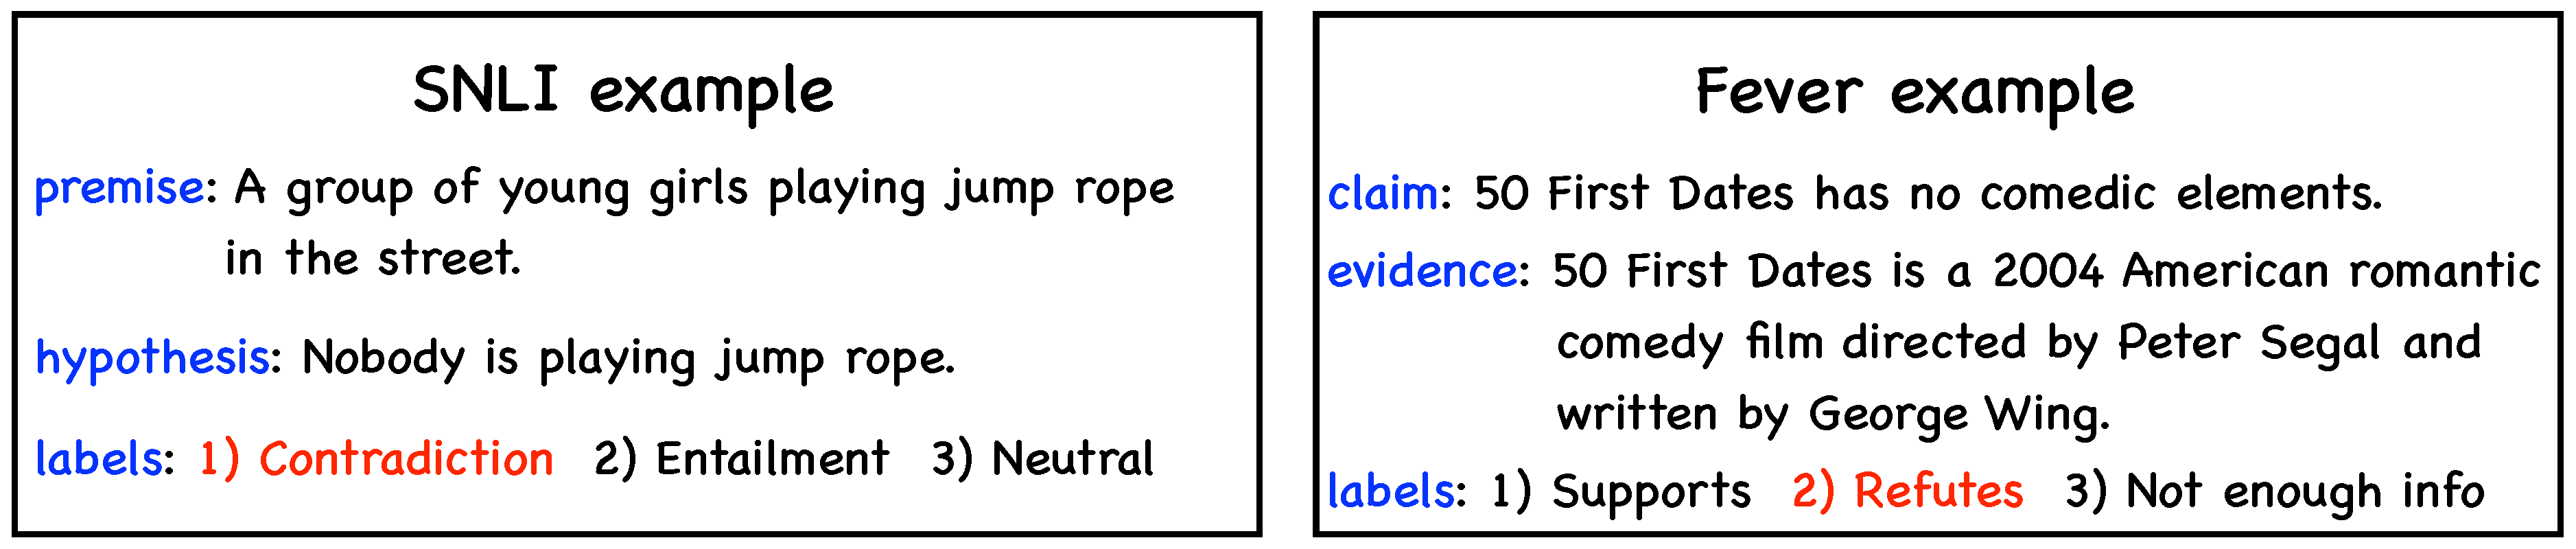
\includegraphics[width=0.9\columnwidth]{figures/noise_example.eps}
	\caption{SNLI and FEVER examples}
	\label{fig:example}
\end{figure}

Benefitting from deeper neutral 
network and larger training data, these models should have a better comprehension 
and reasoning ability. Yet these deep models struggle when taken out of these dataset environments and evaluated
on adversarial data or problems out of domain~\cite{naik2018stress,mccoy2019right,schuster2019towards,nie2019adversarial},
%\YZ{What do you mean by these data? You use spurious cues in abstract and use spurious features in intro, are they same? What is spurious features or cues?}
%which indicates that those datasets overestimate the true capabilities of current models due to spurious features 
%existing in datasets.
%\YZ{
which indicates that the true capabilities of existing models are overestimated due to superficial patterns in current datasets. 
%For example a suspicion phenomenon is that even without premise 
%in NLI tasks or evidence in FEVER, 
%the models can still have a pretty good performance.%\KZ{Give some examples from other papers. Not just cite.}
%}

Superficial pattern analysis in datasets has attracted some attention lately. 
Some work~\cite{gururangan2018annotation,zellers2018swag} 
has shown that many models can even 
get good results without even looking at the stem of the multiple choice questions.
There are mainly two typical types of superficial patterns~\cite{naik2018stress,mccoy2019right,schuster2019towards,nie2019adversarial} observed 
in three datasets, SNLI~\cite{bowman2015large}, MNLI~\cite{williams2018broad} and FEVER: 
%lexicalized and unlexicalized~\cite{}.
%Lexicalized feature Unlexicalized features 
%\KZ{Are you sure ``heuristics'' is the right word??''
%And how many types are there anyway? I'm a bit confused. You should say type 1 is ...;
%type 2 is ... and give an example for each type.}
type 1 is shallow n-gram distribution patterns which mainly contain the indicator of n-gram tokens. 
type 2 is overlap features involving lexical overlap, 
subsequence overlap and constituent overlap~\cite{mccoy2019right} 
assuming that a premise entails all
hypotheses constructed from words
in the premise.% \KZ{Isn't this a repetition of the previous statement? In addition, } 
These spurious features can impact the generalization 
and robustness of models~\cite{bras2020adversarial}.

%we further investigate
%the lexicalized irregularities, what we refer as spurious tokens which can mostly 
%change the result of instances. 
Existing techniques to improve the quality of the datasets 
include data filtering and data augmentation.  
The data filtering model~\cite{bras2020adversarial} 
produces a reduced dataset with
an iterative greedy algorithm that adversarially filters out data points to
identify a reduced dataset with fewer spurious features. 
The greedy algorithm works through getting iteratively 
training results of complex neural network models, like BERT and RoBERTa, . 
%\KZ{I don't get how you can reduce the data thru iteratively training. Be more
%specific?}
%\YZ{You mean that the data filtering models produces a new dataset by complex neural based model?}
However, the down side is this method remove much useful training materials as well
(as much as 90\% of the original data could be removed) and affecting performance on original test set.
%\KZ{Why does data augmentation have to be manual?} 
Most reasoning classification data are unnaturally, since human don't 
always give reasoning alternatives, especially wrong alternatives, in daily life.
Thus a direct data augmentation method is to collect more data manually to remedy 
issues in original datasets. But it consumes a lot and very hard. The new data should meet the form of 
the task and have to solve previous problems. There is still no guarantee that the new data set have 
no new problems~\cite{williams2018broad}.
Thus, some work~\cite{mccoy2019right,min2020syntactic,wang2019if} resorts to automatic generation of 
more adversarial examples to neutralizes some superficial patterns using predefined rules. 
But rules can themselves become the source of new spurious features~\cite{jia2017adversarial,ribeiro2018semantically,iyyer2018adversarial,liu2019inoculation}.
%\KZ{Isn't our method also a kind of such rules? Why doesn't it generate spurious features
%itself?}

In this paper, we propose a new data augmentation method
to enhance the robustness, called noise data augmentation. 
It also aims to generate adversarial examples by making small 
perturbations to the input designed to significantly increase 
the loss incurred by a machine learning model. Different with the 
augmentation methods we mentioned above, we won't introduce 
perturbations into original relational labels directly. Instead, we create 
a new type of examples with a ``Noise'' label. 
The examples of ``Noise'' type are ill-formatted and do not make
grammatical sense. The new label ``Noise'' corresponds to a new relation between the \textit{premise} and \textit{hypothesis} that indicates the given example is a broken one.
For example, we provide examples without premise 
in NLI-like tasks which can be identified as ``Noise'' data. The details will be described 
in~\secref{sec:approach}. In fact, 
we transfer original task to another one which require the model to 
have both the ability of commonsense reasoning and judging what is ``Noise''. 
%by disregarding the simple spurious features 
%and turning to focus more on other more meaningful and perhaps more sophisticated features. . 
%The ``noise'' here carries a different meaning than traditional sense in machine learning
%which usually refers to data examples with incorrect labels.
% \KZ{Give a noise example here.}
The reason we design noises this way is because we aim to avoid 
introducing new spurious features into original task. Even if models learn the spurious 
features in the new ``Noise'' examples, it won't give extra superficial information 
for reasoning test (test without label ``Noise''). This is inspired by the thinking of joint learning.
%For the SNLI example in~\figref{fig:example}, we will never choose ``Entailment'' 
%for the original instance as a new noise sample because this is wrong.
Together with the original examples of the dataset, we come up with an augmented dataset
which we call noise dataset. 
%\YZ{It is not clear. noise examples, original examples? You mean you add noise instances into dataset?}
%In the case of NLI or fact verification datasets, or between \textit{claim} and \textit{evidence} 
%that indicates the given example is a broken because either the example doesn't 
%have a \textit{premise} or a \textit{evidence}. 
%\YZ{Give an example of instance with label Noise ?}
Our goal of augmenting the data is to optimize 
%\YZ{maybe another word is better. How about ``optimize''?}                       
the model by increasing the difficulty of training so that the model cannot be easily
fit with shallow spurious features and focuses on more complex features.

%\KZ{I think u don't wanna keep mentioning hypo (or claims), as if this work only
%targets these two tasks. No! this work should work for more task. We just use
%the two as example. So you should use a single, more general term to refer to them.}  
According to unbalanced token distribution, overlap superficial patterns we 
mentioned above and the phenomenon of hypothesis-only,
%\KZ{Previously you said 2 types, now is 3? Overlap and hypo-only are two or
%three patterns? Make it clear!}, 
we generate noise data from three aspects. 
First, we balance the frequency of tokens in original dataset with new examples.
The generated ones are only a set of words that are not even coherent sentences. 
Models can not easily make decisions only for the appearance of words. 
Second, we random replace some words in \textit{hypothesis}
with words in \textit{premise}
to simulate tokens overlap in an example. 
For example, we take ``playing rope are bad nobody with church 
you when the a.'' as the new premise of a noise example which shares ``playing'', ``rope'' and ``nobody'' 
with \textit{hypothesis} ``Nobody is playing jump rope.''
%\KZ{Again mention hypo and claim: 
Third, we add hypothesis-only noise intuitively to lead model not to recruit
features only from ending.
% These three methods can give more training data with an extra label ``Noise". 
%We try different types and proportions of noise data augmentation.
The models retrained on our new augmentation data 
don't affect performance on the original test set 
%have a consistent performance on 
%original test dataset datasets 
and outperform the models which are trained without noise data
on challenging adversarial datasets~\secref{sec:dataset}. 
%The models retrained on our new augmentation data 
%don't impact performance on the original test set, and outperform 
%the models trained on original or challenging adversarial datasets?
%original dataset and stress test \YZ{original test set and stress test set? Do you need explain what stress test is?}, which 
%shows the retrained models are more robust.with the model 
%trained on original 
%We generate premise-hypothesis pairs with label "Noise" automatic 
%by random choosing a premise and generate a hypothesis with random 
%choose some some words from the whole corpus beyond grammar. 
%We also control the sentence length with average length in original dataset.

%\KZ{Can you crystalize your contributions again?}
%Our contribution of this paper can be summarized in
%two-fold:

%1) We can only consider the frequency, which means the words frequency in 
%our generation part will be equal to the max number in each original labeled part.

%2) We can just delete the premise

%3) We can  change the ending order 


